\documentclass{standalone}
\usepackage{tikz}
\usetikzlibrary{patterns, positioning}


\begin{document}
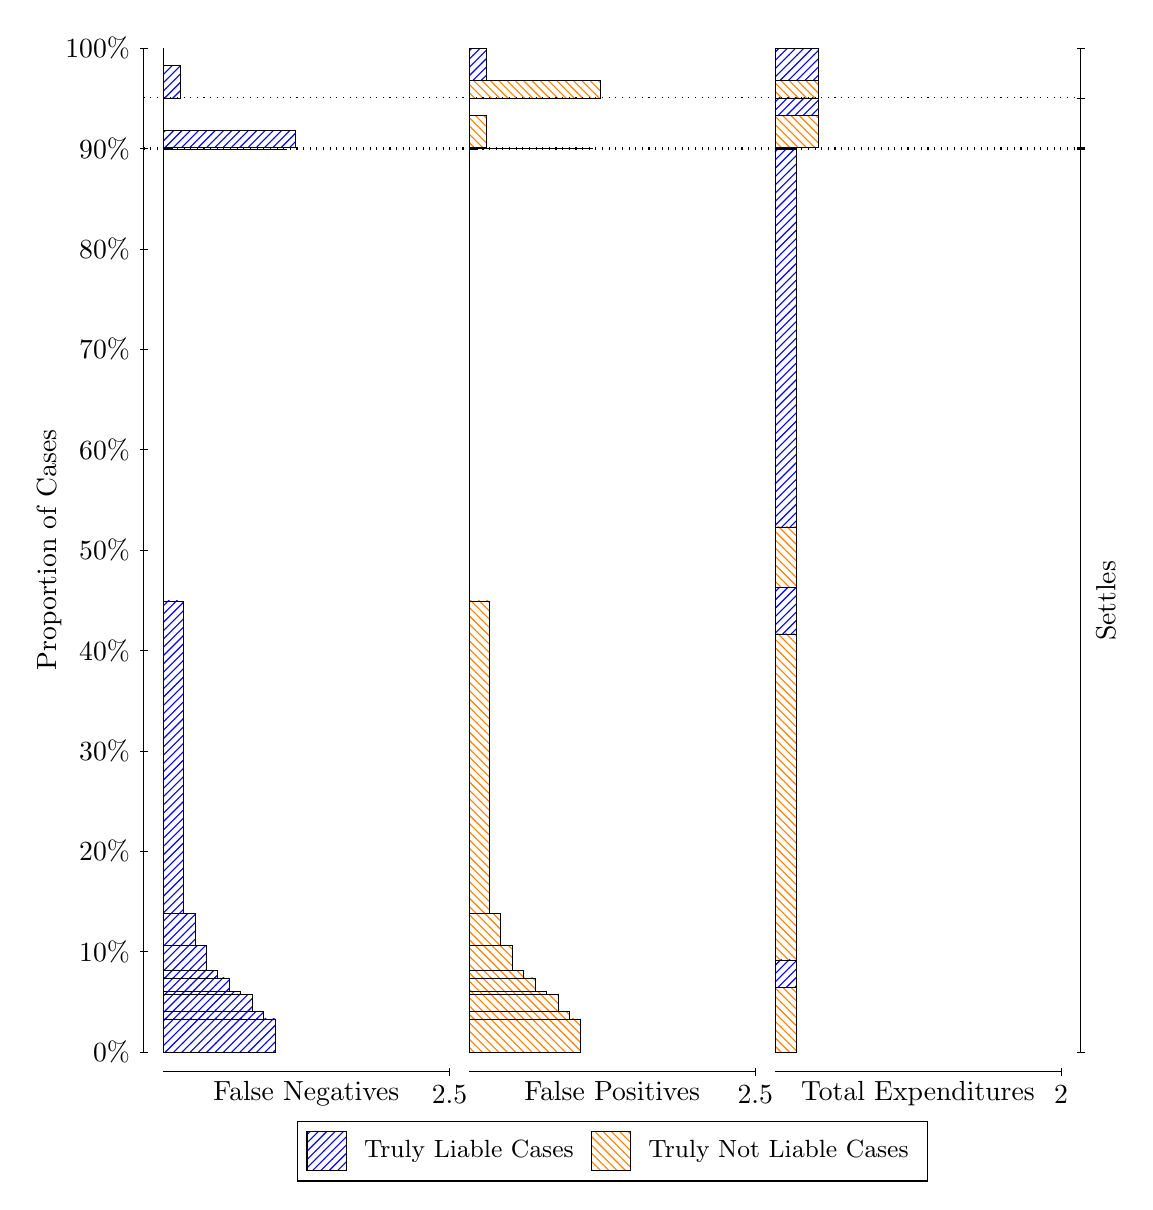
\begin{tikzpicture}
\draw[black, very thin] (1.5,1.75) -- (1.5,14.5);
\node[rotate=90, text=black, anchor=center] at (0.3, 8.125) {Proportion of Cases};
\draw[black, very thin] (1.45,1.75) -- (1.55,1.75);
\node[text=black, anchor=east] at (1.45, 1.75) {0\%};
\draw[black, very thin] (1.45,3.025) -- (1.55,3.025);
\node[text=black, anchor=east] at (1.45, 3.025) {10\%};
\draw[black, very thin] (1.45,4.3) -- (1.55,4.3);
\node[text=black, anchor=east] at (1.45, 4.3) {20\%};
\draw[black, very thin] (1.45,5.575) -- (1.55,5.575);
\node[text=black, anchor=east] at (1.45, 5.575) {30\%};
\draw[black, very thin] (1.45,6.85) -- (1.55,6.85);
\node[text=black, anchor=east] at (1.45, 6.85) {40\%};
\draw[black, very thin] (1.45,8.125) -- (1.55,8.125);
\node[text=black, anchor=east] at (1.45, 8.125) {50\%};
\draw[black, very thin] (1.45,9.4) -- (1.55,9.4);
\node[text=black, anchor=east] at (1.45, 9.4) {60\%};
\draw[black, very thin] (1.45,10.675) -- (1.55,10.675);
\node[text=black, anchor=east] at (1.45, 10.675) {70\%};
\draw[black, very thin] (1.45,11.95) -- (1.55,11.95);
\node[text=black, anchor=east] at (1.45, 11.95) {80\%};
\draw[black, very thin] (1.45,13.225) -- (1.55,13.225);
\node[text=black, anchor=east] at (1.45, 13.225) {90\%};
\draw[black, very thin] (1.45,14.5) -- (1.55,14.5);
\node[text=black, anchor=east] at (1.45, 14.5) {100\%};

\draw[black, very thin] (13.4,1.75) -- (13.4,14.5);
\draw[black, very thin] (13.35,1.75) -- (13.45,1.75);
\node[anchor=west] at (13.35, 1.75) {};
\draw[black, very thin] (13.35,13.208) -- (13.45,13.208);
\node[anchor=west] at (13.35, 13.208) {};
\draw[black, very thin] (13.35,13.221) -- (13.45,13.221);
\node[anchor=west] at (13.35, 13.221) {};
\draw[black, very thin] (13.35,13.234) -- (13.45,13.234);
\node[anchor=west] at (13.35, 13.234) {};
\draw[black, very thin] (13.35,13.867) -- (13.45,13.867);
\node[anchor=west] at (13.35, 13.867) {};
\draw[black, very thin] (13.35,14.5) -- (13.45,14.5);
\node[anchor=west] at (13.35, 14.5) {};

\draw[black, very thin, pattern color=blue, pattern=north east lines] (1.75,1.75) rectangle (3.167,2.1696);
\draw[black, very thin, pattern color=blue, pattern=north east lines] (1.75,2.1696) rectangle (3.0217,2.2621);
\draw[black, very thin, pattern color=blue, pattern=north east lines] (1.75,2.2621) rectangle (2.8763,2.4786);
\draw[black, very thin, pattern color=blue, pattern=north east lines] (1.75,2.4786) rectangle (2.731,2.5217);
\draw[black, very thin, pattern color=blue, pattern=north east lines] (1.75,2.5217) rectangle (2.5857,2.6899);
\draw[black, very thin, pattern color=blue, pattern=north east lines] (1.75,2.6899) rectangle (2.4403,2.787);
\draw[black, very thin, pattern color=blue, pattern=north east lines] (1.75,2.787) rectangle (2.295,3.101);
\draw[black, very thin, pattern color=blue, pattern=north east lines] (1.75,3.101) rectangle (2.1497,3.5065);
\draw[black, very thin, pattern color=blue, pattern=north east lines] (1.75,3.5065) rectangle (2.0043,7.4791);
\draw[black, very thin, pattern color=orange, pattern=north west lines] (1.75,7.4791) rectangle (1.75,13.208);
\draw[black, very thin, pattern color=blue, pattern=north east lines] (1.75,13.208) rectangle (3.3123,13.209);
\draw[black, very thin, pattern color=orange, pattern=north west lines] (1.75,13.209) rectangle (1.75,13.221);
\draw[black, very thin, pattern color=blue, pattern=north east lines] (1.75,13.221) rectangle (1.859,13.232);
\draw[black, very thin, pattern color=orange, pattern=north west lines] (1.75,13.232) rectangle (1.75,13.234);
\draw[black, very thin, pattern color=blue, pattern=north east lines] (1.75,13.234) rectangle (3.4213,13.457);
\draw[black, very thin, pattern color=orange, pattern=north west lines] (1.75,13.457) rectangle (1.75,13.867);
\draw[black, very thin, pattern color=blue, pattern=north east lines] (1.75,13.867) rectangle (1.968,14.277);
\draw[black, very thin, pattern color=orange, pattern=north west lines] (1.75,14.277) rectangle (1.75,14.5);
\draw[black, very thin, pattern color=orange, pattern=north west lines] (5.6333,1.75) rectangle (7.0503,2.1696);
\draw[black, very thin, pattern color=orange, pattern=north west lines] (5.6333,2.1696) rectangle (6.905,2.2621);
\draw[black, very thin, pattern color=orange, pattern=north west lines] (5.6333,2.2621) rectangle (6.7597,2.4786);
\draw[black, very thin, pattern color=orange, pattern=north west lines] (5.6333,2.4786) rectangle (6.6143,2.5217);
\draw[black, very thin, pattern color=orange, pattern=north west lines] (5.6333,2.5217) rectangle (6.469,2.6899);
\draw[black, very thin, pattern color=orange, pattern=north west lines] (5.6333,2.6899) rectangle (6.3237,2.787);
\draw[black, very thin, pattern color=orange, pattern=north west lines] (5.6333,2.787) rectangle (6.1783,3.101);
\draw[black, very thin, pattern color=orange, pattern=north west lines] (5.6333,3.101) rectangle (6.033,3.5065);
\draw[black, very thin, pattern color=orange, pattern=north west lines] (5.6333,3.5065) rectangle (5.8877,7.4789);
\draw[black, very thin, pattern color=blue, pattern=north east lines] (5.6333,7.4789) rectangle (5.6333,13.208);
\draw[black, very thin, pattern color=orange, pattern=north west lines] (5.6333,13.208) rectangle (5.7423,13.22);
\draw[black, very thin, pattern color=blue, pattern=north east lines] (5.6333,13.22) rectangle (5.6333,13.221);
\draw[black, very thin, pattern color=orange, pattern=north west lines] (5.6333,13.221) rectangle (7.1957,13.222);
\draw[black, very thin, pattern color=blue, pattern=north east lines] (5.6333,13.222) rectangle (5.7423,13.234);
\draw[black, very thin, pattern color=orange, pattern=north west lines] (5.6333,13.234) rectangle (5.8513,13.644);
\draw[black, very thin, pattern color=blue, pattern=north east lines] (5.6333,13.644) rectangle (5.6333,13.867);
\draw[black, very thin, pattern color=orange, pattern=north west lines] (5.6333,13.867) rectangle (7.3047,14.09);
\draw[black, very thin, pattern color=blue, pattern=north east lines] (5.6333,14.09) rectangle (5.8513,14.5);
\draw[black, very thin, pattern color=orange, pattern=north west lines] (9.5167,1.75) rectangle (9.7892,2.5666);
\draw[black, very thin, pattern color=blue, pattern=north east lines] (9.5167,2.5666) rectangle (9.7892,2.9187);
\draw[black, very thin, pattern color=orange, pattern=north west lines] (9.5167,2.9187) rectangle (9.7892,7.0593);
\draw[black, very thin, pattern color=blue, pattern=north east lines] (9.5167,7.0593) rectangle (9.7892,7.6471);
\draw[black, very thin, pattern color=orange, pattern=north west lines] (9.5167,7.6471) rectangle (9.7892,8.4188);
\draw[black, very thin, pattern color=blue, pattern=north east lines] (9.5167,8.4188) rectangle (9.7892,13.208);
\draw[black, very thin, pattern color=orange, pattern=north west lines] (9.5167,13.208) rectangle (9.7892,13.22);
\draw[black, very thin, pattern color=blue, pattern=north east lines] (9.5167,13.22) rectangle (9.7892,13.221);
\draw[black, very thin, pattern color=orange, pattern=north west lines] (9.5167,13.221) rectangle (9.7892,13.222);
\draw[black, very thin, pattern color=blue, pattern=north east lines] (9.5167,13.222) rectangle (9.7892,13.234);
\draw[black, very thin, pattern color=orange, pattern=north west lines] (9.5167,13.234) rectangle (10.062,13.644);
\draw[black, very thin, pattern color=blue, pattern=north east lines] (9.5167,13.644) rectangle (10.062,13.867);
\draw[black, very thin, pattern color=orange, pattern=north west lines] (9.5167,13.867) rectangle (10.062,14.09);
\draw[black, very thin, pattern color=blue, pattern=north east lines] (9.5167,14.09) rectangle (10.062,14.5);
\draw[black, dotted] (1.5,13.208) -- (13.4,13.208);
\draw[black, dotted] (1.5,13.221) -- (13.4,13.221);
\draw[black, dotted] (1.5,13.234) -- (13.4,13.234);
\draw[black, dotted] (1.5,13.867) -- (13.4,13.867);
\draw[black, very thin] (1.75,1.5) -- (5.3833,1.5);
\node[text=black, anchor=north] at (3.5667, 1.5) {False Negatives};
\draw[black, very thin] (5.3833,1.45) -- (5.3833,1.55);
\node[text=black, anchor=north] at (5.3833, 1.45) {2.5};

\draw[black, very thin] (5.6333,1.5) -- (9.2667,1.5);
\node[text=black, anchor=north] at (7.45, 1.5) {False Positives};
\draw[black, very thin] (9.2667,1.45) -- (9.2667,1.55);
\node[text=black, anchor=north] at (9.2667, 1.45) {2.5};

\draw[black, very thin] (9.5167,1.5) -- (13.15,1.5);
\node[text=black, anchor=north] at (11.333, 1.5) {Total Expenditures};
\draw[black, very thin] (13.15,1.45) -- (13.15,1.55);
\node[text=black, anchor=north] at (13.15, 1.45) {2};

\node[text=black, centered, rotate=90] at (13.72, 7.479) {Settles};





\draw (7.449999999999999,1.5) node[draw=none] (baseCoordinate) {};
\begin{scope}[align=center]
        \matrix[scale=0.5, draw=black, below=0.5cm of baseCoordinate, nodes={draw}, column sep=0.1cm]{
            \node[rectangle, draw, minimum width=0.5cm, minimum height=0.5cm, pattern color=blue, pattern=north east lines] {}; &
            \node[draw=none, font=\small, text=black] (B) {Truly Liable Cases}; &
            \node[rectangle, draw, minimum width=0.5cm, minimum height=0.5cm, pattern color=orange, pattern=north west lines] {}; &
            \node[draw=none, font=\small, text=black] (B) {Truly Not Liable Cases}; \\
            };
\end{scope}

\end{tikzpicture}
\end{document}